

\documentclass[conference]{IEEEtran}
\ifCLASSINFOpdf
   \usepackage[pdftex]{graphicx}
\else

\fi
\usepackage[cmex10]{amsmath}
\usepackage{amssymb}
\usepackage{wrapfig}
\usepackage{url}
\usepackage[caption=false,font=footnotesize]{subfig}
\hyphenation{op-tical net-works semi-conduc-tor}

\usepackage{subscript}



\begin{document}


\title{KNN classifier with self adjusting memory for heterogenous concept drift }


\author{\IEEEauthorblockN{Viktor Losing\IEEEauthorrefmark{1}\IEEEauthorrefmark{2},
Barbara Hammer\IEEEauthorrefmark{1} and
Heiko Wersing\IEEEauthorrefmark{2}}
\IEEEauthorblockA{\IEEEauthorrefmark{1}Bielefeld University, Universit\"atsstr. 25, 33615 Bielefeld}
\IEEEauthorblockA{\IEEEauthorrefmark{2}HONDA Research Institute Europe, Carl-Legien-Str. 30, 63073 Offenbach am Main}
}



\maketitle


\setcounter{figure}{0}
\begin{abstract}
Learning from non-stationary data streams is gaining more attention
recently, especially in the context of Internet of Things and Big Data.
It is a highly challenging task, since the fundamentally different types
of possibly occurring drift undermine classical assumptions such as
i.i.d data. Incremental drift characterizes a continuous change in the
distribution such as the signals of a slowly degrading sensor. A
suddenly malfunctioning sensor on the other hand causes a severe shift
and is defined as abrupt drift. Available algorithms are able to handle
different types of drift, however they target either abrupt or
incremental drift and often incorporate hyperparameter requiring a
priori knowledge about the task at hand.\\
We propose a biological inspired, architecture which partitions the data
into a short-term and long-term memory. The former is a window of
recently seen data-points whose size is adjusted such that the estimated
generalization error is minimized. The latter preserves only those
information from previous concepts which are non-conflicting to the
current one. These memories are combined according to the demands of the
present concept to classify unseen data points. We couple our parameter
free approach with the K-Nearest Neighbor classifier, however, any other
incremental learning algorithm could be used as well. \\
New artificial and real datasets are proposed to evaluate performance on
specific types of drift. Experiments on these as well as on generally
known benchmark datasets compare our approach with state of the art
methods. The highly competitive results throughout all experiments
underline the robustness of our approach.
\end{abstract}

\IEEEpeerreviewmaketitle

\section{Introduction}
\section{Concept Drift}
Definition and examples
\subsection{Types of Drift}
-abrupt, incremental, gradual, reoccuring, virtual
\section{Related Work}
-Survey by gamma eventuell Ditzler
-Active drift detection work Gamma, Bifet ADWIN for abrupt to minimize delay
-Passive drift handling with ensembles DACC, LPPNSE
-Windowing but usually throws away information which still can be valid, no LTM
  -SVM Leave one out
  -KNNPAW 
-KNN for streaming like the ICDM paper


\section{Architecture}
Our architecture is depicted in figure \ref{XXVL}. It consists of 4 different steps. The goal is to keep as much as possible of the current concept in the Short Term Memory(STM) and at the same
time preserve former knowledge in the Long Term Memory (LTM). We assume that the recent information is correct and reflects the current concept. Therefore, it is crucial to make
sure that the memory in the LTM is not conflicting. 

\subsection{Short Term Memory}
-STM, partitioning, O(log n) tests, maximizing generalization accuracy, write down in fancy formal way
-LTM, keep not compromising
-Transfer
-choosing of proper prediction model(STM, or LTM, or Both)
-Clustering
-Size management

\subsection{Efficiency}
-distances have to be calculated anyways once, can be stored and afterwards need only to be sorted
-fits with other algorithms as long they can be trained incremental and decremental e.g. NB, incremental SVM, but how to solve validation procedure
-approximative KNN
-adapt stm not every example but every n examples

\section{Experiments}
We compare our method with well-known state of the art methods for handling drifting streaming data. Implementations of the original authors or those available in MOA \cite{bifet2010moa}
have been used to conduct the experiments. The following algorithms are considered in the evaluation:\\
\\\textbf{Learn++.NSE}\\
Proposed in \cite{5975223}, this algorithm processes incoming samples in chunks with a predefined size. A base classifier is trained for each chunk and added to the ensemble. The loss on recent chunks is averaged with a sigmoidal function
to compute the final weight of each base classifier. Similar to AdaBoost, instances are weighted such that misclassified inputs have a higher impact on the calculated loss.
Chunk-wise trained models have by design an adaption delay depending on the chunk size. The base classifier are in our case Classification and Regression Trees \cite{cart84}.
\\\textbf{Leveraging Bagging}\\
Bifet et al. propose in \cite{bifet2010leveraging} to increase the randomization of Online Bagging \cite{oza2005online} and thereby the diversity of the ensemble.
This is done by a higher $\lambda$ value for the poisson distribution and the usage of output detection codes. Additionaly, they use ADWIN as change detector for every classifier within the ensemble such that whenever a change is detected 
the worst classifier is replaced by a new one. Hoeffding Trees\cite{domingos2000mining} with Gaussian Naive Bayes within the leaves are used as base classifier.
XXVL maybe define Hoeffding trees.
\\\textbf{Dynamic Adaption of Concept Changes}\\
Within this ensemble algorithm \cite{jaber2013online} a classifier of the worst half of the pool is removed randomly after a predefined number of examples and replaced by a new one. 
Newly generated classifier are excluded for a predefined time from the elimination process. Incoming examples are solely classified by the classifier within the pool which
achieved the highest accuracy in the past. As in Leavarging Bagging, Hoeffding Trees were the base classifier within the pool.
\\\textbf{kNN with Sliding Window}\\
This classifier is a kNN with a fixed window size containing the most recent samples. The sliding window is a standard approach for drift handling, since the window contains usually the most relevant examples
for the future predictions. However, since the size is static the window may contain outdated examples interfering with the current concept leading to a deterioration of the prediction accuracy. 
\\\textbf{kNN with Probabilistic Adaptive Window and ADWIN}\\
In contrast to the approach with the sliding window, examples are here removed randomly leading to a window which not only contains recent samples but also older ones. The window size is not bounded strictly
and varies around a target size (see \cite{Bifet:2013:EDS:2480362.2480516}). This approach also uses ADWIN for change detection and clears the window accordingly. \\
Table \ref{tab:algorithms} gives an overview of the algorithms as well as the chosen hyperparameter. 
\begin{table}
\def\arraystretch{0.9}
\footnotesize
\centering
\caption{The compared algorithms.}
\label{tab:algorithms}
\begin{tabular}{l|cccc}
\textit{Abbr.} & Classifier & Parameter\\\hline
HT\textsubscript{A} & Hoeffding Tree with ADWIN \\
LPPNSE & Learn++.NSE with CART& chunk-Size = various\\
DACC & Dynamic with HT& n=10\\
LVGB & Leveraging Bagging with HT& n=10\\
KNN\textsubscript{S} & KNN with sliding window & w=5000, k=5\\
KNN\textsubscript{W\textsubscript{A}} & NN with PAW+ADWIN& w=5000, k=5\\
KNN\textsubscript{M} &KNN with STM+LTM memory & w=5000, k=5\\
\end{tabular}
\end{table}
A maximum of 5000 samples was allowed as size for the window based approaches. However,
we limited it to at most 10\% of the whole dataset for those with rather few examples. LPPNSE demands a chunk size which is critical for its performance. To avoid any disadvantage 
we evaluated several sizes and report the best result. No further dataset specific hyperparameter tuning was done, as we wanted to use as little prior knowledge as possible.

\subsection{Datasets}
We used own and well known artificial as well as real world datasets to compare our method with state of the art algorithms. 
Links to all datasets as well as our own ones are available at \url{https://github.com/vlosing/Online-learning}. In the following we describe the data more detailed.\\

Artificial datasets have the advantage that any desired drift behavior can be explicitly simulated to analyze certain properties of a given method. These are often 
2-dimensional and to enable a straightforward visualization. We evaluated ready to use published benchmark datasets as well as MOA generated ones using common parametrization in the literature.
We also added four new datasets allowing the evaluation of particular algorithm properties which are in our opinion not yet considered enough in the community. 
Table \ref{tab:artDatasets} shows their main characteristics.
\begin{table}
\caption{Evaluated artificial datasets.}
\label{tab:artDatasets}
\centering
\begin{tabular}{l|cccc}
\textit{Dataset} & \#Samples&\#Feat.&\#Class&Drift type\\\hline
SEA Concepts & 50K & 3 & 2 & abrupt\\
Rotating Hyperplane & 200K & 10 & 2 & incremental\\
Moving RBF & 200K & 10 & 5 & incremental\\
Interchanging RBF & 200K & 2 & 10 & abrupt\\
Moving Squares & 200K & 2 & 4 & incremental\\
Transient Chessboard & 200K & 2 & 8 & virtual\\
Mixed Drift & 600K & 2 & 8 & abr/incr/virt\\
\end{tabular}
\end{table}
\\\textbf{SEA Concepts (SEA)}\\
This two class dataset was proposed in \cite{Street:2001:SEA:502512.502568} and consists of 50000 samples with three attributes of which only two are relevant.
Abrupt drift is simulated with four different concepts, changing every 12500 samples, by using different thresholds $\theta_i$ such that $f_1 + f_2 > \theta_i$.
This dataset includes 10\% of noise.\\
\textbf{Rotating Hyperplane (HYP)}\\
A hyperplane in d-dimensional space is defined by the set of points $x$ that satisfy $\sum_{i=1}^{d}w_ix_i=w_0$. The position and orientation of the hyperplane
are changed incrementally by continuously adding a term $\delta$ to the weights $w_i=w_i+\delta$. 
We used the generator in MOA with the same parameters as in \cite{Bifet:2013:EDS:2480362.2480516} (10 dimensions, 2 classes, $\delta$=0.001).\\ 
\textbf{Moving RBF (MRBF)}\\
Gaussian distributions with random initial positions, weight and standard deviations are moved with constant speed $v$ in d-dimensional speed. 
The weight controls the partitioning of all samples among the Gaussians.
We used the generator in MOA with the same parameters as in \cite{Bifet:2013:EDS:2480362.2480516} (10 dimensions, 50 Gaussians, 5 classes, $v$=0.001).\\ 
\textbf{Interchanging RBF (IRBF)}\\
Ten Gaussians with random covariance matrix are exchanging positions every $2000$ samples and generate thereby a total of 100 abrupt drifts.\\ 
\textbf{Moving Squares (SQR)}\\
Four equidistantly seperated squares, representing different classes, are moving in horizontal direction with constant speed. The direction is inverted whenever the leading squares reaches a predefined boundary.
The nice property of this dataset is that the upper bound of stored recent examples such that old samples do not overlap current ones can be easily calculated (120) and  
facilitates the analysation of algorithms, especially those using a sliding window approach, for incremental drift.\\
\textbf{Transient Chessboard (CHESS)}
This dataset simulates virtual drift by succesively revealing random squares of a chessboard. Each time after four squares have been revealed, samples covering all squares of the board are shown.
facilitating the classification for algorithms which preserve as much information as possible.\\ 
\textbf{Mixed Drift (MIX)} \\
The datasets interchanging RBF, moving squares and transient chessboard datasets are simply positioned next to each other and samples belonging to one of these are introduced alternately.
Therefore, incremental, abrupt and virtual drift are taking place at the same time, requiring local adaptation to different drift types.\\

Unfortunately, only a few real world drift benchmarks are available, of which we used the largest ones. Additionaly, we contributed two challenging new datasets obtained from visual data.
The main attributes of all considered real world datasets are given in Table \ref{tab:realDatasets}.
\begin{table}
\caption{Considered real world datasets. The given drift type was determined as described in \ref{driftType}.}
\label{tab:realDatasets}
\centering
\begin{tabular}{l|cccc}
\textit{Dataset} & \#Samples&\#Feat.&\#Class&Drift type\\\hline
\rule{0pt}{8pt}
Weather & 18159 & 8 & 2 & virtual\\
Elec & 27549 & 6 & 2 & real\\
CovType & 581012 & 54 & 784 & real\\
Outdoor & 4000 & 21 & 40 & real\\
Railto & 40000 & 27 & 10 & real\\
\end{tabular}
\end{table}
\\\textbf{Weather}\\
Elwell et al. introduced this dataset in \cite{5975223}. Using eight different features such as temperature, pressure wind speed etc. the target is to predict 
whether it is going to rain on a certain day or not at the Offutt Air Force Base in Bellevue, Nebraska.
A period of 50 years is covered (1949-1999) summing up to 18159 samples with an imbalance towards no rain ($69\%$).\\
\textbf{Electricity market dataset}\\
This problem is often used as a benchmark for concept drift classification. Initially described in \cite{harries1999splice}, it was used thereafter for several performance comparisons \cite{baena2006early}, \cite{kuncheva2008adaptive}, \cite{Bifet:2013:EDS:2480362.2480516}, \cite{gama2004learning}. 
A critical note to its suitability as a benchmark can be found in \cite{zliobaite2013good}.
The dataset holds information of the Australian New South Wales Electricity Market, whose prices are affected by supply and demand. 
Each sample characterized by attributes such as day of week, timestamp, market demand etc. refers to a period of 30 minutes and the class label identifies the relative change (higher or lower) compared to the last 24 hours.
The dataset is often termed ELEC2 and contains 45312 samples. However, we removed those with missing values leading to a total of 27449 points.\\
\textbf{Forest Cover Type}\\
Assigns cartographic variables such as elevation, slope, soil type asf of $30 \times 30$ meter cells to different forest cover types. 
Only forests with minimal human-caused disturbances were used, so that resulting forest cover types are more a result of ecological processes.
It is often used as a benchmark for drift algorithms \cite{Bifet:2013:EDS:2480362.2480516}, \cite{gama2003accurate}, \cite{oza2001experimental}.\\
\textbf{Outdoor Objects}\\
This visual dataset was obtained from images recorded by a mobile robot approaching 40 different objects in a garden environment \cite{losing2015interactive}. The lighting conditions between 
the approaches are varying significantly caused by different weather conditions and/or cast shadows making the classification quite challenging. Each approach
consists of 10 images and is represented in temporal order within the dataset. Even though the representation is quite stable during a single approach, there is a change of varying degree between different
approaches of the same object XXVL pictures. The objects are encoded in a normalized 21-dimensional rg-chromaticity histogram.\\
\textbf{Railto Bridge Timelapse}\\
Ten of the colorful buildings next to the famous rialto bridge in Venice are encoded in a normalized 27-dimensional rgb histogram. 
The images were obtained from timelapse videos of 10 consecutive days recorded in may 2016 by a webcam of XXVL. Continuously changing weather and lighting conditions affect the representation  XXVL see figures. We excluded overnight recordings since they were too dark for being useful.
\subsubsection{Assessing the drift type in real world data}\label{driftType}
While the drift is explicitly generated in artificial datasets, it is rather difficult to identify the drift type or whether drift is present at all in real world datas. Therefore, it is usually
assumed in the comunity that there is some drift contained in the commonly evaluated datasets. We propose in this section a method which is able to determine the present drift type in a 
given dataset. To the best of our knowledge this has not been done so far in literature. Our two staged approach can distinguish between real, virtual or no drift at all. 
In the first step we are able to conclude whether real drift is present. If that is not the case, we continue with the second step which detects virtual drift. 
Whenever both tests are negative we infer that no drift is present at all. We heavily use sliding windows of various sizes for this analysis. 
The type of classifier is interchangeable, however, we used once again KNN.\\


The idea for the first step is inspired by the observation that whenever real drift is present, sliding windows of smaller sizes tend to deliver higher accuracies than larger ones. 
This contradicts the classical assumption for i.i.d datasets, backed up by the PAC theory(XXVL reference!), that the more data is stored in a model the less mistakes are done. 
However, streaming data is not i.i.d and more mistakes are done whenever outdated data from former concepts is in conflict with samples of the current one. 
A window which contains less of the outdated samples, delivers therefore a better result. 

XXVL mention online learning accuracy.
We propose to test whether the accuracies achieved with sliding windows of different sizes are significantly higher than the one obtained without any size restriction. 
To obtain multiple accuracies for a given window side we generate bootstrapped samples of the dataset maintaining the initial order. 
Afterwards, we perform a one sided hypothesis test with the traditional p-value of 5\%.
The method is described exemplarly for one window size s1 in the following.\\
Given a dataset X with n examples, we generate b bootstrap samples $\Psi=\hat{X}_1,\hat{X}_2...{X}_b$of the dataset and sort them such that the initial order in the dataset is preserved. 
We train a classifier with window size $s_1$ and another one with $s_n$ using $\Psi$ and asses their accuracies $a_1,a_2,...a_b$ and $\tilde{a}_1,\tilde{a}_2,...\tilde{a}_b$ respectively.  
The pth percentile of all accuracy differences $d_i = a_i - \tilde{a}_i$ is calculated. The null hypothesis, accuracy $a_i <= \tilde{a}_i$, is rejected if its value is smaller 0.\\
In case of no real drift, we proceed with the second step and test for virtual drift. Here we permutate the dataset each time before generating the bootstrapped samples and compare
the resulting accuracies with those obtained in the first stage using the same window size. The permutation mixes data of all concepts. If P(X) is changed over time an 
algorithm should achieve higher accuracies, since it is easier to classify only one concept at a time instead of all of them together.\\
Next to the real world data we also analyzed the drift type of artificial data as a proof of concept. We used 200 bootstrap samples per window size.
Table \ref{tab:drifttype} shows the mean accuracies of the bootstrapped samples with corresponding standard deviations and the inferred drift type. Our approach classifies correctly
the drift type of all artificial datasets. In the case of the artificial datasets the increase/decrease of performance with shrinking window sizes is quite significant for datasets
with / without real drift. This is generally less pronounced for real real world data. Nonthelss, the datasets Elec, Outdoor and Rialto clearly benefit from smaller window sizes. 
Covtype contains little real drift, while the Weather task incorporates only virtual drift.
\begin{table*}
\caption{Mean accuracies and corresponding standard deviations obtained from bootstrapped samples of the datasets with varying sliding window sizes.}
\label{tab:drifttype}
\centering
\subfloat[Bootstrapped samples for detecting real drift. Accuracies of size restricted windows which are significantly higer compared to the accuracy achieved without restriction are marked bold. 
If this is the case at least for one window size it is inferred that the dataset contains real drift.]{
\begin{tabular}{l|ccccccc}
\textit{Dataset} & KNN\textsubscript{S-100}&KNN\textsubscript{S-500}&KNN\textsubscript{S-1000}&KNN\textsubscript{S-5000}&KNN\textsubscript{S-10000}&KNN&Concluded drift type\\\hline
Weather              &82.03(0.12)&84.05(0.24)&84.36(0.25)&84.95(0.18)&84.92(0.20)&84.86(0.16)&not real\\
Elec                 &\textbf{89.08(0.18)}&\textbf{87.46(0.17)}&\textbf{86.61(0.16)}&\textbf{85.07(0.11)}&\textbf{84.22(0.14)}&83.43(0.13)&real\\
CovType              &94.65(0.01)&96.15(0.01)&\textbf{97.11(0.01)}&\textbf{96.95(0.01)}&\textbf{96.92(0.01)}& 5&real\\
Outdoor              &89.08(0.18)&87.46(0.17)&86.61(0.16)&85.07(0.11)&84.22(0.14)&83.43(0.13)&real\\
Railto               &89.08(0.18)&87.46(0.17)&86.61(0.16)&85.07(0.11)&84.22(0.14)&83.43(0.13)&real\\\hline
Chessboard i.i.d.    &63.23(0.07)&83.63(0.07)&88.47(0.06)&94.67(0.03)&96.15(0.04)&98.37(0.02)& not real\\
Transient Chessboard &81.00(0.05)&88.56(0.04)&88.85(0.04)&94.81(0.02)&95.89(0.03)&98.36(0.03)& not real\\
Moving Squares       &\textbf{97.73(0.02)}&\textbf{67.22(0.05)}&\textbf{63.30(0.05)}&56.87(0.11)&57.22(0.04)&57.12(0.10)& real\\
Interchanging RBF    &97.73(0.02)&67.22(0.05)&63.30(0.05)&56.87(0.11)&57.22(0.04)&57.12(0.10)& real\\
\end{tabular}
}
\par\vspace{5 pt}
\subfloat[Permutated bootstrapped samples for detecting real drift. Accuracies which are significantly higher compared to those achieved in a) 
with the same window size are marked bold and it is assumed that the corresponding dataset incorporates virtual drift]{
\begin{tabular}{l|ccccccc}
\textit{Dataset} & KNN\textsubscript{S-100}&KNN\textsubscript{S-500}&KNN\textsubscript{S-1000}&KNN\textsubscript{S-5000}&KNN\textsubscript{S-10000}&KNN&Concluded drift type\\\hline
\rule{0pt}{8pt}
Weather              &\textbf{81.14(0.30)}&\textbf{83.20(0.23)}&83.89(0.28)&84.42(0.17)&84.77(0.19)&84.63(0.18)&virtual\\\hline
Chessboard i.i.d.    &63.25(0.05)&83.63(0.06)&88.44(0.06)&94.71(0.04)&96.18(0.02)&98.36(0.01)&None\\
Transient Chessboard &\textbf{63.30(0.09)}&\textbf{83.77(0.06)}&\textbf{88.48(0.05)}&94.77(0.03)&96.20(0.05)&98.38(0.02)&virtual\\
\end{tabular}
}

\end{table*}

\subsection{Results}
We evaluated the algorithms in the standard online learning setting in which each incoming example is first classified and afterwards used for training. The error rates of all experiments are shown
in Table \ref{tab:result}.\\
\begin{table*}
\caption{Error rates of all experiments evaluated with the Interleaved Test-Then-Train method.}
\label{tab:result}
\centering
\begin{tabular}{l|ccccccc}
Dataset & HT\textsubscript{A} & LPPNSE &DACC& LVGB & kNN\textsubscript{S} & kNN\textsubscript{W\textsubscript{A}}& kNN\textsubscript{M}\\\hline
SEA & 13.8 & 10.00 & 10.00 & 10.00 & 10.00 & 10.00 & 10.00\\
HYP & 10.00 & 10.00 & 10.00 & 10.00 & 10.00 & 10.00 & 10.00\\ 
MRBF & 10.00 & 10.00 & 10.00 & 10.00 & 10.00 & 10.00 & 10.00\\
IRBF & 10.00 & 10.00 & 10.00 & 10.00 & 10.00 & 10.00 & 10.00\\
SQR & 10.00 & 10.00 & 10.00 & 10.00 & 10.00 & 10.00 & 10.00\\
CHESS & 10.00 & 10.00 & 10.00 & 10.00 & 10.00 & 10.00 & 10.00\\
MIX & 10.00 & 10.00 & 10.00 & 10.00 & 10.00 & 10.00 & 10.00\\\hline
Art. avg & 10.00 & 10.00 & 10.00 & 10.00 & 10.00 & 10.00 & 10.00\\\hline
Art. rank & 10.00 & 10.00 & 10.00 & 10.00 & 10.00 & 10.00 & 10.00\\\hline
Weather & 10.00 & 10.00 & 10.00 & 10.00 & 10.00 & 10.00 & 10.00\\
Elec & 10.00 & 10.00 & 10.00 & 10.00 & 10.00 & 10.00 & 10.00\\
CovType & 10.00 & 10.00 & 10.00 & 10.00 & 10.00 & 10.00 & 10.00\\
Outdoor & 10.00 & 10.00 & 10.00 & 10.00 & 10.00 & 10.00 & 10.00\\
Railto & 10.00 & 10.00 & 10.00 & 10.00 & 10.00 & 10.00 & 10.00\\\hline
Real avg& 10.00 & 10.00 & 10.00 & 10.00 & 10.00 & 10.00 & 10.00\\\hline
Real rank& 10.00 & 10.00 & 10.00 & 10.00 & 10.00 & 10.00 & 10.00\\\hline
total avg& 10.00 & 10.00 & 10.00 & 10.00 & 10.00 & 10.00 & 10.00\\\hline
total rank& 10.00 & 10.00 & 10.00 & 10.00 & 10.00 & 10.00 & 10.00\\\hline
\end{tabular}
\end{table*}
(XXVL name of algorithm) outperforms the other algorithms quite significantly by having nearly half the error rate in average compared to the second best method LVGB. 
Even more important is in our eyes the fact that while all other methods are struggling at some datasets our aproach delivers very robust results without any hiccup. All drift types are handled
better or at least competitive compared to the other algorithms. This is particularly clarified in the large accuracy gap achieved with the MIX dataset, which contains incremental, 
abrupt and virtual drift at the same time. \\
The methodically most similar method to ours is kNN\textsubscript{W\textsubscript{A}}, since it uses also kNN as classifier and actively manages its window.
However, it performs in all experiments worse, even in those containing only abrupt drift.\\
Our results confirm the fact that kNN is in general a very competitive algorithm in the streaming setting. It is quite surprising that the simple sliding window approach of fixed window size
kNN\textsubscript{S} performs comparably well or even better than more sophisticated methods such as HTAdaptive or L++.NSE.

\subsection{Memory behaviour}
In this section we illustrate the behavior of the STM and LTM during the experiments in a detailed way. 
Figure \ref{fig:abrupt} depicts the size adjustment of the STM in case of abrupt drift using the dataset XXVL. 
\begin{figure}
\centering
	\subfloat{%
	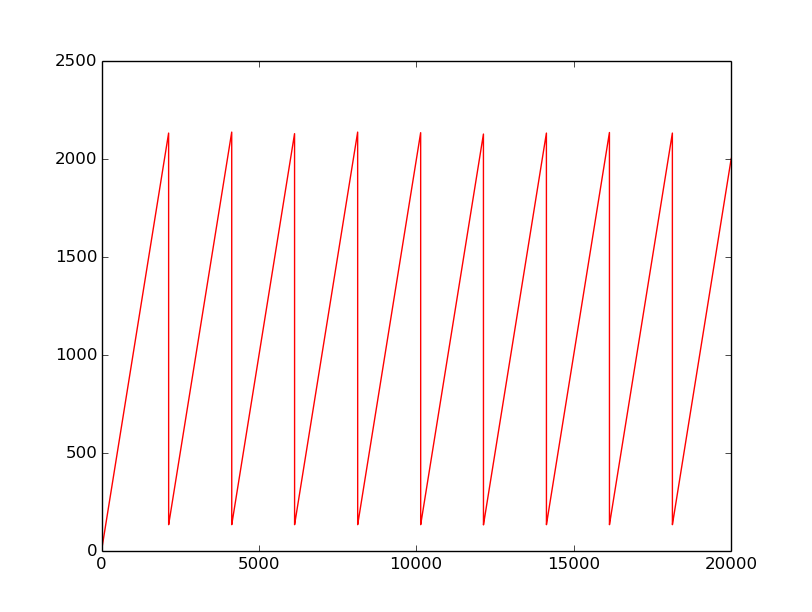
\includegraphics[width=0.24\textwidth]{images/abruptSTMSize.png}
	}
	\subfloat{%
	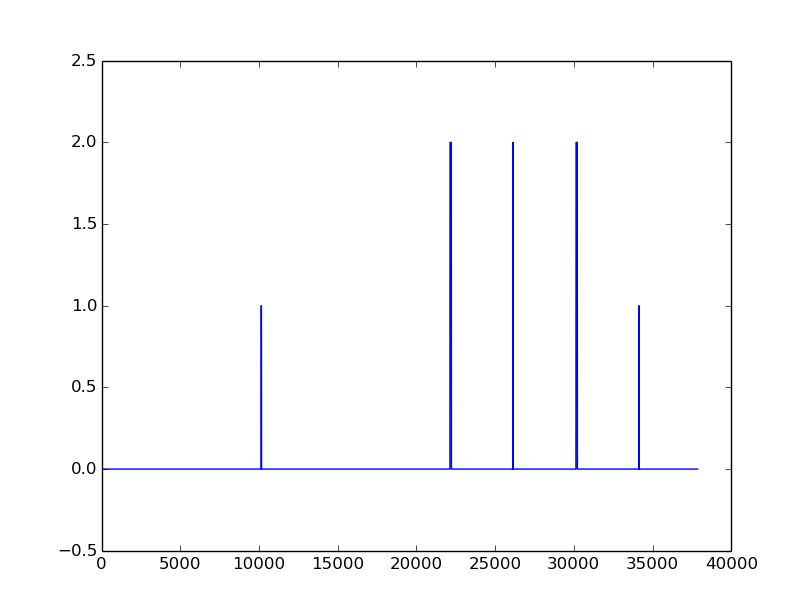
\includegraphics[width=0.24\textwidth]{images/abruptResp.png}
	}
	\vspace{0 pt}
	\subfloat{%
	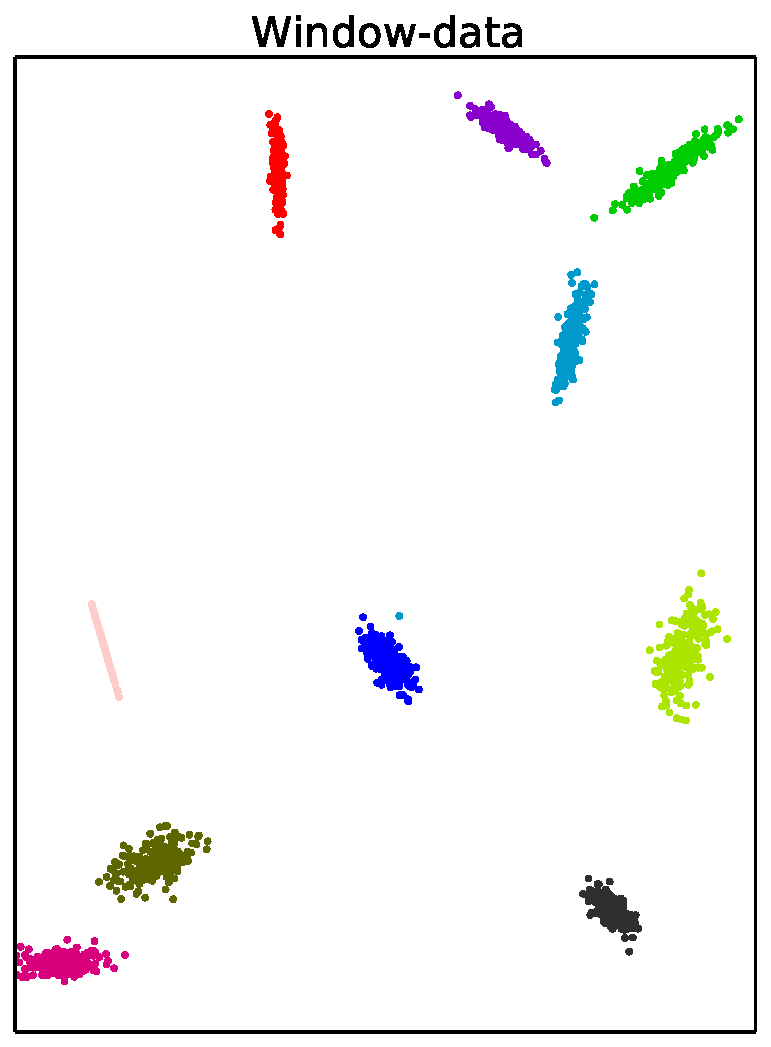
\includegraphics[width=0.24\textwidth]{images/abruptSTM.pdf}
	}
	\subfloat{%
	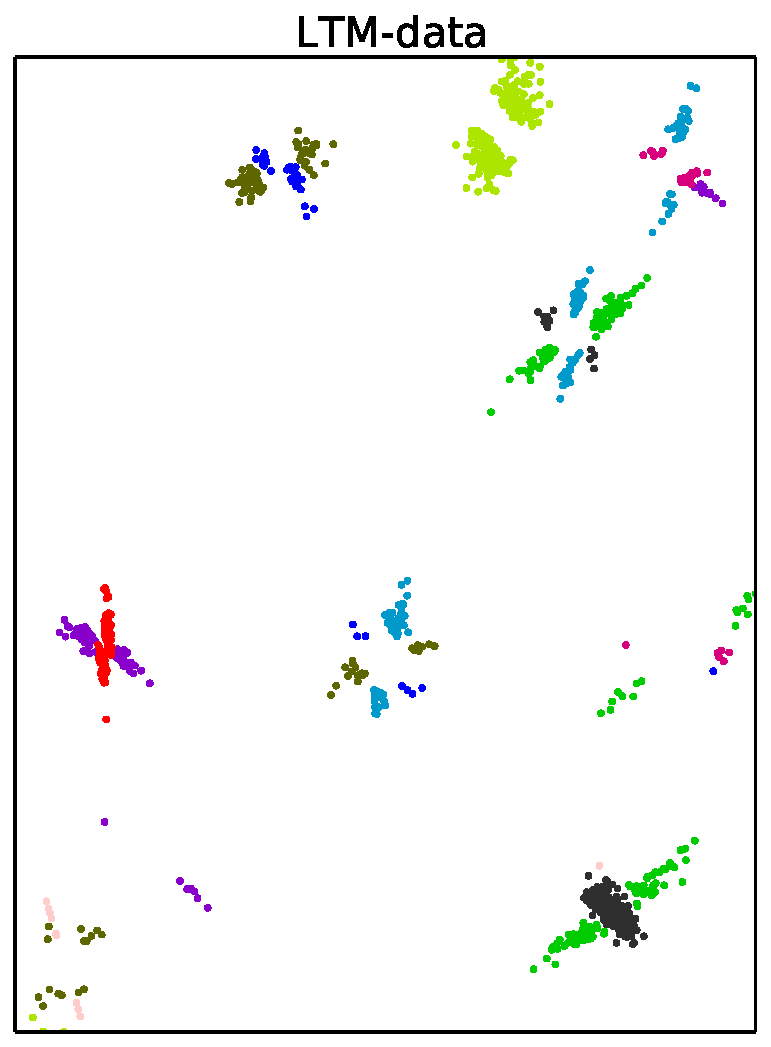
\includegraphics[width=0.24\textwidth]{images/abruptLTM.pdf}
	}
\label{fig:abrupt}
\caption{}
\end{figure}
The algorithm shrinks the window reliably each time after an abrupt drift occurs.
However, we can also observe that there is each time a certain delay until the memory is shrinked properly during which false predictions may occur. 
This delay is due to two reasons. Firstly, a certain amount of examples of the new concept is required to be able to construct a reliable classifier for it. Secondly,
the more examples were contained in the short term memory before the new concept, the more stable was the classifier and the more examples of the 
new concept are required to deteriorate its accuracy until the the new classifier performs better. Therefore, the behavior illustrates a natural trade-off between adaption speed
to new concepts and the robustness against noise, governed by the stability of the concepts.\\
The consolidation of the LTM is also visible in Figure \ref{fig:abrupt}. All samples interfering with the STM deleted, and therefore the feature space is empty there. 
Whereas the samples around the empty spots do not conflict with the STM and kept in the memory.\\
As already mentioned the Moving Squares dataset is constructed in such a way that the squares may start to overlap if more than one 120 samples are kept in the memory. Hence,
for this dataset the best strategy is to use only the most recent examples for prediction and keep the memory as small as possible. 
Figure \ref{fig:squares} shows the behavior of the STM for this dataset. 
\begin{figure}
\centering
	\subfloat{%
	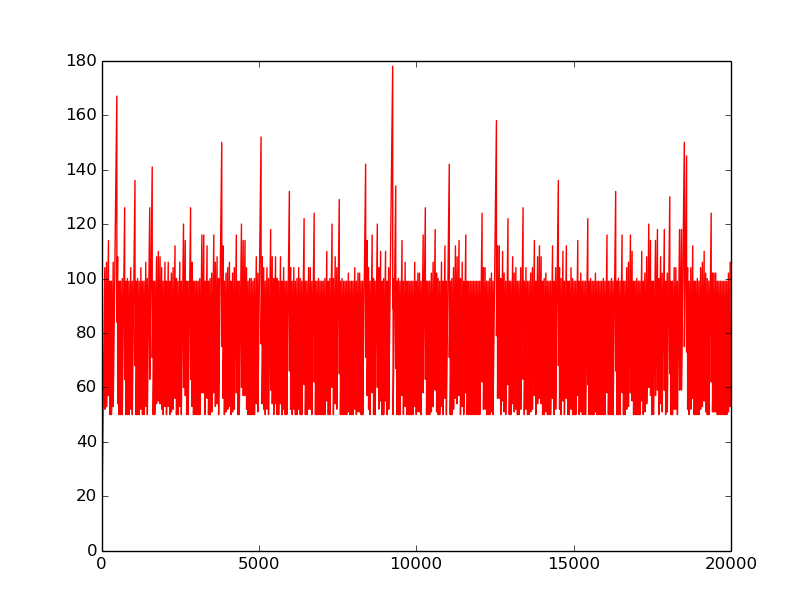
\includegraphics[width=0.24\textwidth]{images/squaresSTMSize.png}
	}
	\subfloat{%
	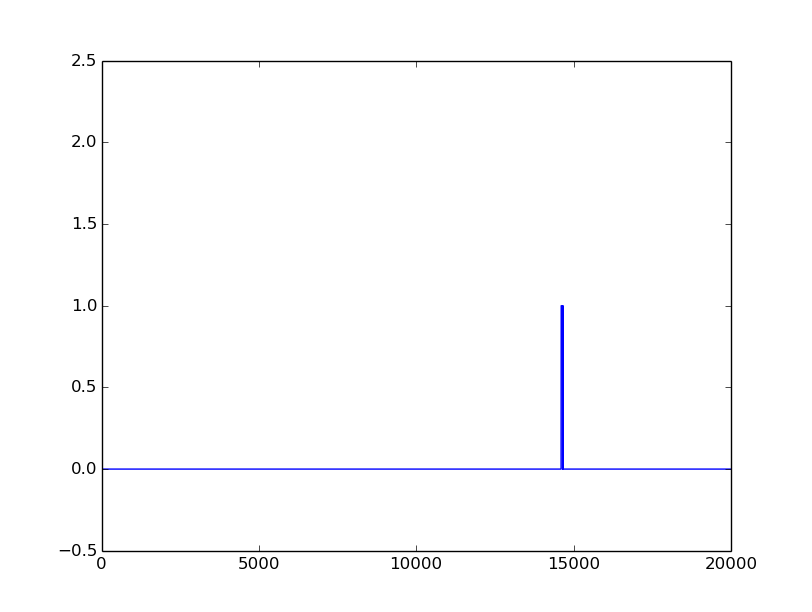
\includegraphics[width=0.24\textwidth]{images/squaresResp.png}
	}
	\vspace{0 pt}
	\subfloat{%
	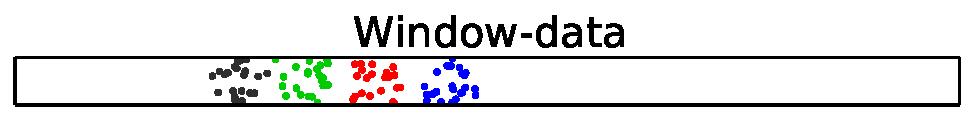
\includegraphics[width=0.24\textwidth]{images/squaresSTM.pdf}
	}
	\subfloat{%
	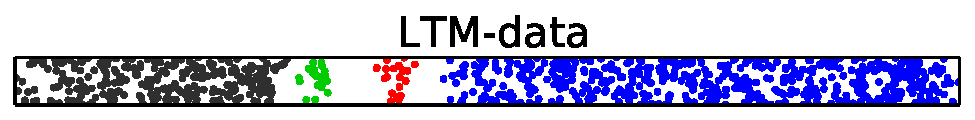
\includegraphics[width=0.24\textwidth]{images/squaresLTM.pdf}
	}
\label{fig:squares}
\caption{}
\end{figure}
Most of the time the memory is kept between 50 and 100 samples, allowing a nearly perfect prediction. 
The reason that the window is mostly shrinked around 100 examples is that the default parameter for the minimal size of the STM is set to 50.\\
The LTM keeps the examples at the borders since these are touched only by one class.\\
The Transient Chessboard dataset uses virtual drift. Figure \ref{fig:chess} shows some plots for this dataset.
\begin{figure}
\centering
	\subfloat{%
	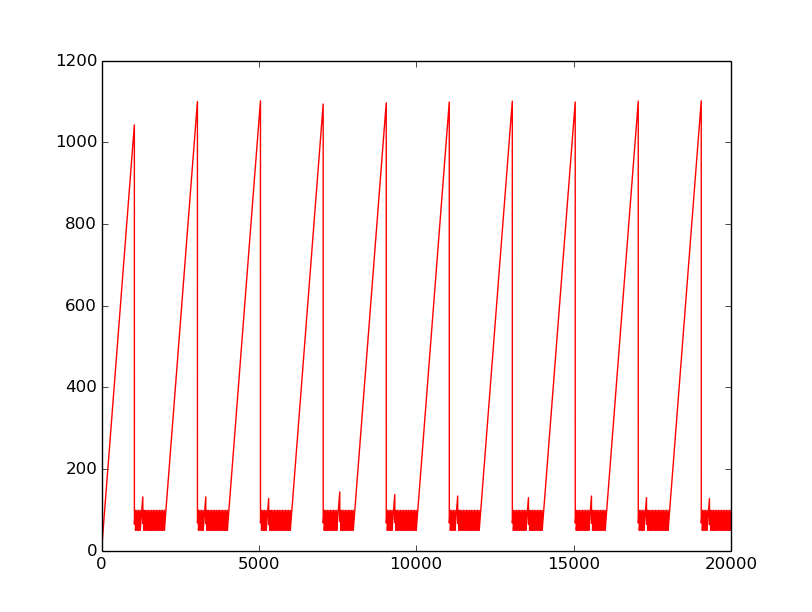
\includegraphics[width=0.24\textwidth]{images/chessSTMSize.png}
	}
	\subfloat{%
	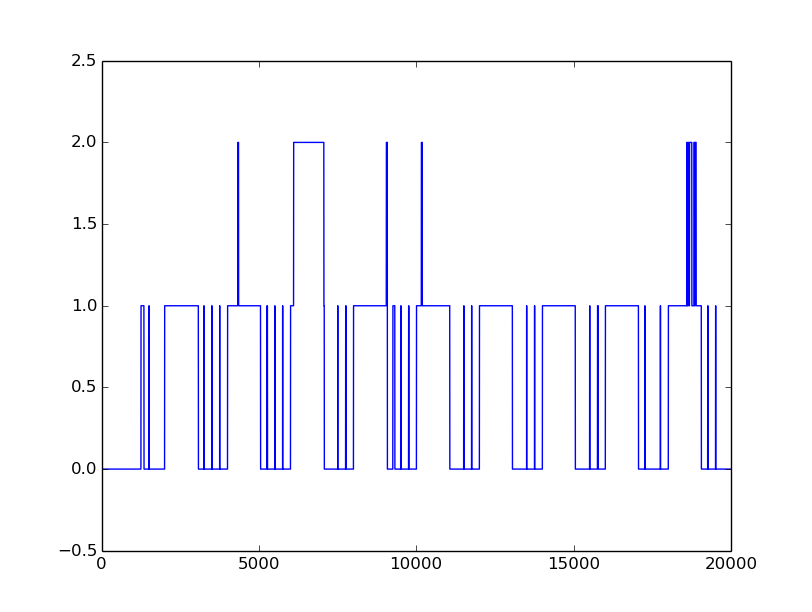
\includegraphics[width=0.24\textwidth]{images/chessResp.png}
	}
	\vspace{0 pt}
	\subfloat{%
	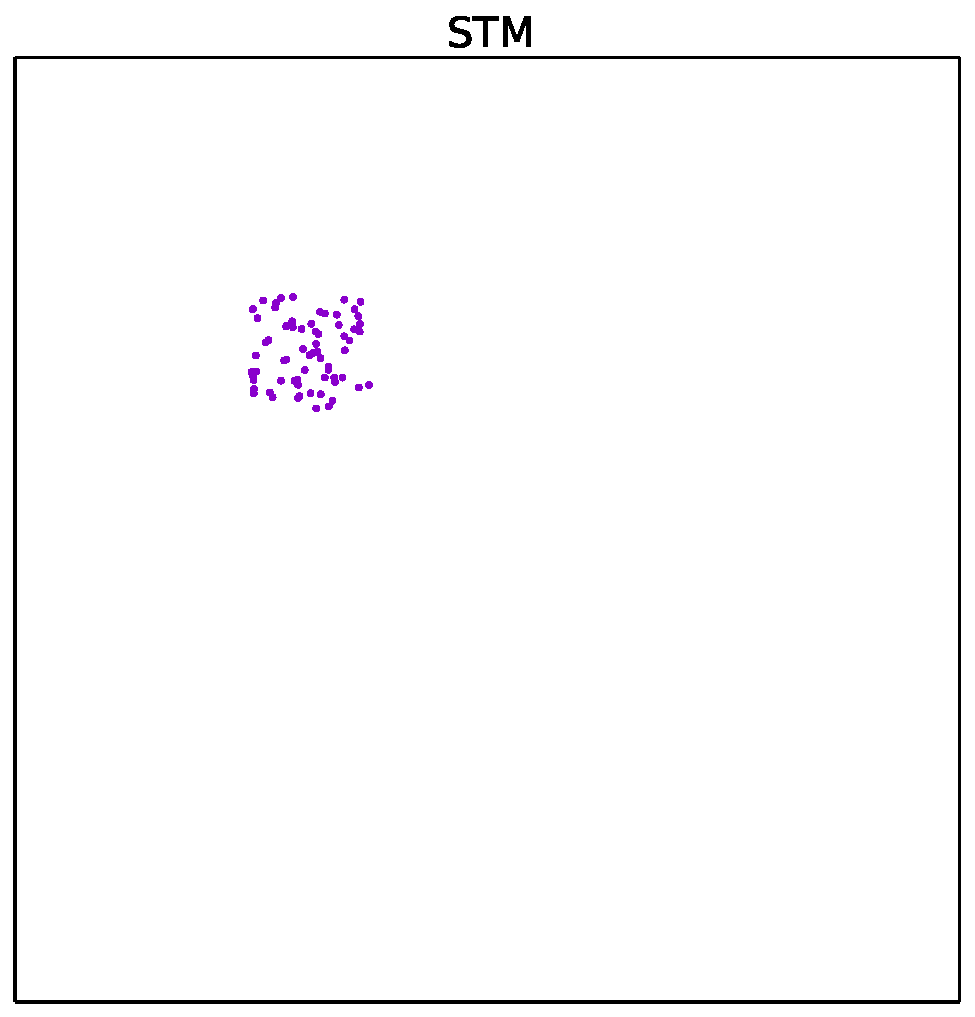
\includegraphics[width=0.24\textwidth]{images/chessSTM.pdf}
	}
	\subfloat{%
	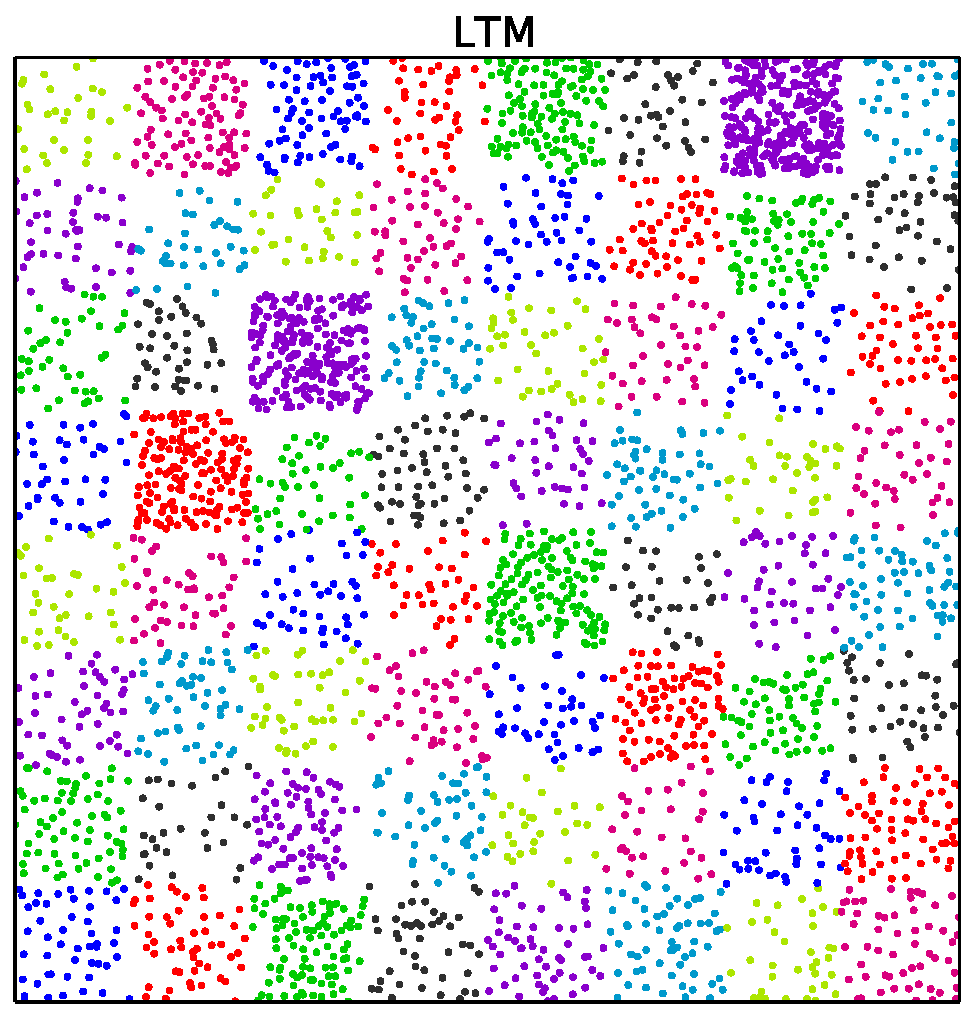
\includegraphics[width=0.24\textwidth]{images/chessLTM.pdf}
	}
\label{fig:chess}
\caption{}
\end{figure}
In contrast to the previous two datasets which basically do not require the LTM, we see here that it 
is often used for the prediction. The STM is used alone whenever
field by field is revealed, since the classification is easier and therefore the accuracy is higher. But as soon as the spray along all fields occurs, the LTM
is heavily used since it contains beneficial information from the past. 

-weather prior, label


\section{Conclusion}

\newpage

% trigger a \newpage just before the given reference
% number - used to balance the columns on the last page
% adjust value as needed - may need to be readjusted if
% the document is modified later
%\IEEEtriggeratref{8}
% The "triggered" command can be changed if desired:
%\IEEEtriggercmd{\enlargethispage{-5in}}

% references section

% can use a bibliography generated by BibTeX as a .bbl file
% BibTeX documentation can be easily obtained at:
% http://www.ctan.org/tex-archive/biblio/bibtex/contrib/doc/
% The IEEEtran BibTeX style support page is at:
% http://www.michaelshell.org/tex/ieeetran/bibtex/
%\bibliographystyle{IEEEtran}
% argument is your BibTeX string definitions and bibliography database(s)
%\bibliography{IEEEabrv,../bib/paper}
%
% <OR> manually copy in the resultant .bbl file
% set second argument of \begin to the number of references
% (used to reserve space for the reference number labels box)
\bibliographystyle{IEEEtran}
\bibliography{IEEEabrv,Drift}

% that's all folks
\end{document}

\iffalse
ToDo:

subfloats labeling Benni fragen
Test-Accuracy in Captions